\section{Computational Methods}
\subsection{Monte-Carlo Procedure}
The Monte Carlo simulations were carried out in Mathematica using  code provided by the UCD Theoretical Condensed Matter
group. The majority of these simulations were carried out on a 16 * 19 lattice giving 1024 islands total. The Monte Carlo procedure is as follows:
\par
\begin{enumerate}
\item Initialisation step where every island is assigned a switching value before the Monte Carlo procedure, given by $H_S = H_0 \epsilon$, where $\epsilon$ is a dimensionless Gaussian random variable with mean 1 and variance $\sigma$. The variance, external field magnitude $H_{Ext}$ and external field angle are input parameters.
\item The dipolar field $H_{dip}$ is calculated before running the Monte Carlo selection using the Ewald summation technique.
\item An island in the lattice is randomly selected using a pseudo-random number generator.
\item The local field at the island is given by:
\begin{equation}
    H_L = \hat{e}_{i} (H_{dip}  + H_{ext}) \ ,
\end{equation}
where $\hat{e}_{i}$ is the unit vector pointing along the anisotropy direction of the island.
\item If the local field at the island exceeds the switching value the island's magnetic moment is flipped. Otherwise, the moment remains unchanged and the process is repeated from step 2.
\end{enumerate}
\par
\begin{figure}[ht!]
    \begin{center}
        \subfloat[Initial test run state][Initial test run state]{
        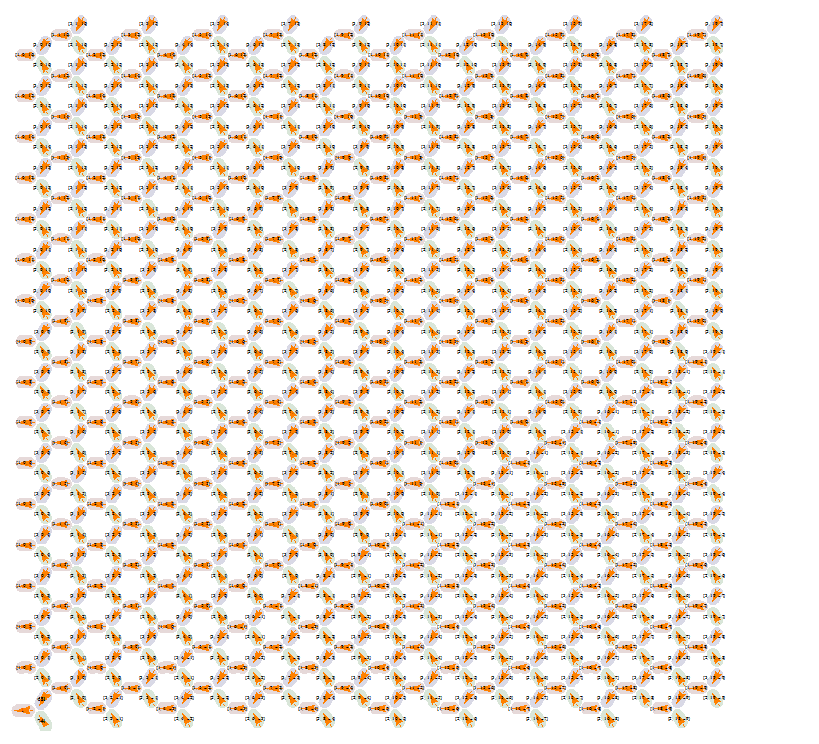
\includegraphics[width=0.40\textwidth]{initpatch.png}
        \label{fig:sf10.1}}
\qquad
        \subfloat[Final test run state][Final test run state]{
        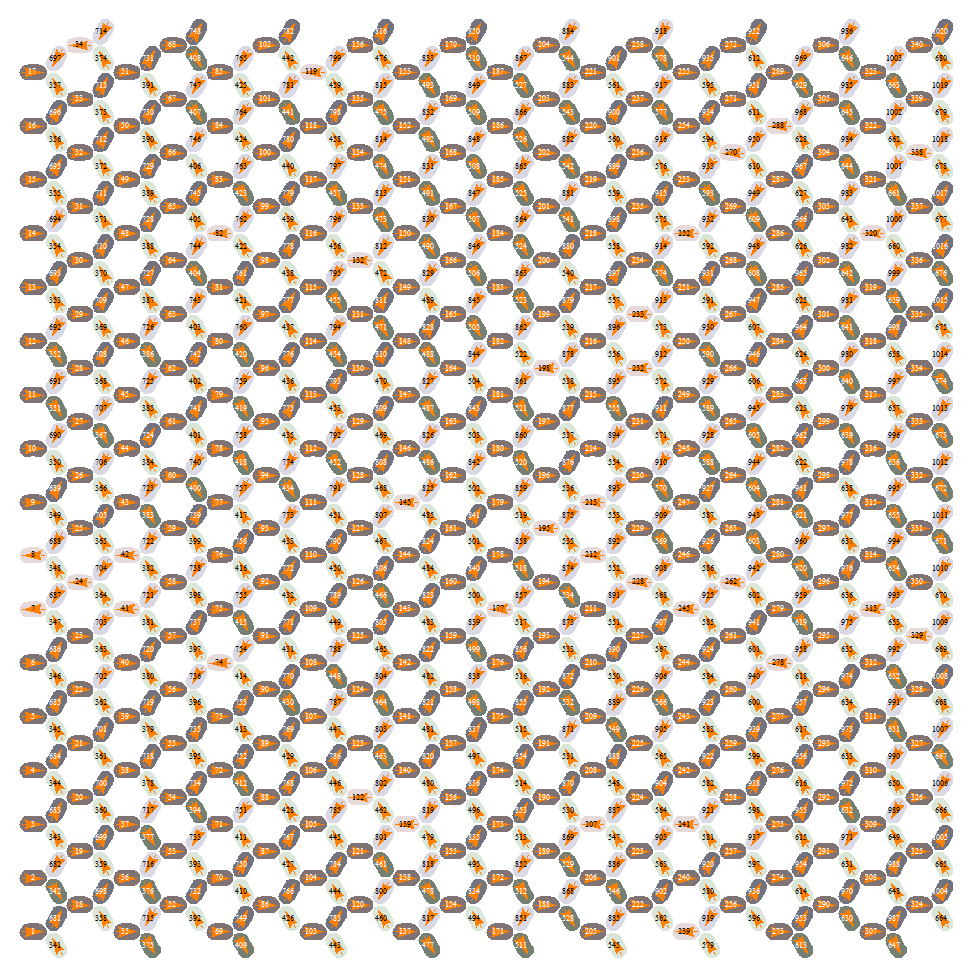
\includegraphics[width=0.37\textwidth]{27run.png}
        \label{fig:sf10.2}}
        \caption[Initial and final test run states]{Initial and final test run states}
        \label{fig:gf10}
    \end{center}
\end{figure}
Steps 2 - 5 are repeated 15n times, where n is the number of islands in the lattice.  The above figure 11(a) shows a typical initial lattice saturated with an external field in the $\theta = 0$ direction. Figure 11(b) is the result of running the Monte Carlo procedure with an external field of 2.7 in the $\theta = 0$ direction and a value for $\sigma$ of 0.13. The dark-coloured islands are ones which have had their magnetic moment flipped.
\par
The parameter $\epsilon$ gives a measure of the strength of each island's anisotropy. Islands with a large value of $\epsilon$ will require a higher field to flip, corresponding physically to islands with a strong anisotropy. Similarly islands with a low $\epsilon$ value correspond physically to islands with a low anisotropy. Thus the variance of $\epsilon$ is a measure of the disorder in the lattice.  If the anisotropy of each island was the same then the lattice would be isotropic and all dipoles would flip at the same value for the magnetic field.
\par
Before each simulation a number of input parameters need to be initialised, such as the magnitude and angle of the external field, the variance of the anisotropies, the initial lattice configuration, etc. Furthermore it was possible to run several simulations consecutively, with a specific parameter varying between
a given initial and final value in a chosen step size.
\subsection{Ewald Summation}
The Ewald summation technique was used to calculate the dipolar fields. It's a standard technique used in the calculation of long range forces on a periodic lattice and is a special case of the Poisson summation formula:
\begin{equation}
    \sum_{n \epsilon \mathbb{R}} f(n) = \sum_{k \epsilon \mathbb{R}} \hat{f}(k) \ ,
\end{equation}
where $\hat{f}$ is the Fourier transform of the function f. The sums over $\mathbb{R}$ can be replaced by discrete sums over $\mathbb{Z}$ and the formula can be generalised to higher dimensions. For example the sums could be taken over a discrete 2-D periodic lattice, as was the case for the simulations performed here. However, it is then
necessary to include a geometric factor $\gamma$ on the right hand side of equation 5.
\par
This depends on the structure of the unit cell used. We shall denote the dipole field at an island i due to a dipole j as $H_{ij}$ . The
patch used in the simulation (a $17 \times 20$ unit kagome lattice with each unit having 3 dipoles amounting to 1020 islands) is replicated periodically, extending the lattice to an infinite size. Thus the dipole field at site i due to site j(m,n), where (m,n) is the location of the island in the infinite lattice, is now denoted $H_{ij}(m,n)$. The total field at i due to dipole j is then given by:
\begin{equation}
    H_{ij} = \sum_{m,n \, \epsilon \, {\mathbb{Z}}^2} H_{ij}(m,n) \ ,
\end{equation}
where the sum is over all periodic patches in the infinite lattice. The total dipolar field at i is thus simply:
\begin{equation}
    H_{i} = \sum_{j=1}^{1020} \left( \sum_{m,n \, \epsilon \, {\mathbb{Z}}^2} H_{ij}(m,n) \right) \ .
\end{equation}
This method is slowly convergent in real space and the need to take a sufficiently large number of terms in order to obtain an accurate result is computationally inefficient.  There is another problem with this as $H_{i,j}$ is dependent on 1/r the convergence is conditional insofar as the order in which the sum is carried out.  We can overcome this problem by using the Poisson Summation to replace equation 6 with:
\begin{equation}
    H_{ij} = \sum_{k,q \, \epsilon \, {\mathbb{Z}}^2} \hat{H}_{ij}(k,q) \ ,
\end{equation}
where $\hat{H}_{ij}$ is the Fourier transform of $H_{ij}(m,n)$.  It is also worth mentioning that we can absorb the geometric factor into $\hat{H}_{ij}$.  The advantage of summing over $\hat{H}_{ij}$ is that the sum is rapidly convergent so an accuracy obtained with previously using equation 7 is obtained with fewer terms to be computed using equation 8.  This is therefore a reduction in computation time to compute accurate fields.
\clearpage
